\setcounter{section}{-1}
\section{Introduction}
	
	%Difficulty
	%This is an introductory workshop.
		
	\subsection*{How to use these booklets}

	The aim of these booklets is to help you attempt these workshops at home, and to explain concepts in more detail than at the workshop. You don't need to follow these booklets during the workshop, but you can if you'd like 0to.
	
	%Code Listings
		The scratch code for this workshop will be shown in the booklet as images like the one shown in \autoref{fig:1followmouse1}.
	
	\begin{figure}[h]
		\centering
		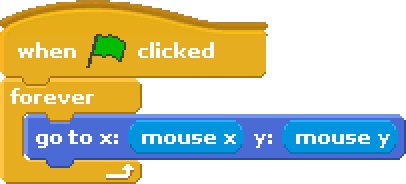
\includegraphics[height=69px]{McrRaspJam/018_ScratchGames/code/1_followmouse1}
		\caption{example code block}
		\label{fig:1followmouse1}
	\end{figure}
	%Occasionally, a concept will be explained in greater detail in \textit{asides}, like the one below. You can read these as you wish, but they're not required to complete the workshop.
	
\begin{aside}[API]
	We use an \textit{Application Programming interface} called `MCPI' to create Python programs for \textit{Minecraft: Pi Edition}.
	
	The API is a set of Python functions which allow us to communicate with the Minecraft game.
\end{aside}

	\subsection*{Everything else}
	
		\iffalse
	
		% Aknowledgements
		These booklets were created using \textrm{\LaTeX}, an advanced typesetting system used for several sorts of books, academic reports and letters.
			
		If you'd like to have a look at using LaTeX, We recommend looking at \TeX studio, which is available on most platforms, and also in the 	Raspbian repository.
		
		\fi
		
		% License spiel
		To allow modification and redistribution of these booklets, they are distributed under the \hbox{CC BY-SA 4.0} License.
		Latex source documents are available at \url{http://github.com/McrRaspJam/booklet-workshops}
		
		If you get stuck, find errors or have feedback about these booklets, please email me at:
		\href{mailto:jam@jackjkelly.com}{\texttt{jam@jackjkelly.com}}